%%%%%%%%%%%%%%%%%%%%%%% file template.tex %%%%%%%%%%%%%%%%%%%%%%%%%
%
% This is a general template file for the LaTeX package SVJour3
% for Springer journals.          Springer Heidelberg 2010/09/16
%
% Copy it to a new file with a new name and use it as the basis
% for your article. Delete % signs as needed.
%
% This template includes a few options for different layouts and
% content for various journals. Please consult a previous issue of
% your journal as needed.
%
%%%%%%%%%%%%%%%%%%%%%%%%%%%%%%%%%%%%%%%%%%%%%%%%%%%%%%%%%%%%%%%%%%%
%
% First comes an example EPS file -- just ignore it and
% proceed on the \documentclass line
% your LaTeX will extract the file if required
\begin{filecontents*}{example.eps}
%!PS-Adobe-3.0 EPSF-3.0
%%BoundingBox: 19 19 221 221
%%CreationDate: Mon Sep 29 1997
%%Creator: programmed by hand (JK)
%%EndComments
gsave
newpath
  20 20 moveto
  20 220 lineto
  220 220 lineto
  220 20 lineto
closepath
2 setlinewidth
gsave
  .4 setgray fill
grestore
stroke
grestore
\end{filecontents*}
%
\RequirePackage{fix-cm}
%
%\documentclass{svjour3}                     % onecolumn (standard format)
%\documentclass[smallcondensed]{svjour3}     % onecolumn (ditto)
\documentclass[smallextended]{svjour3}       % onecolumn (second format)
%\documentclass[twocolumn]{svjour3}          % twocolumn
%
\smartqed  % flush right qed marks, e.g. at end of proof
%
\usepackage{graphicx}
%
% \usepackage{mathptmx}      % use Times fonts if available on your TeX system
%
% insert here the call for the packages your document requires
%\usepackage{latexsym}
% etc.
%
% please place your own definitions here and don't use \def but
% \newcommand{}{}
%
% Insert the name of "your journal" with
% \journalname{myjournal}
%
\begin{document}

\title{Breast milk on the go:%\thanks{Grants or other notes
%about the article that should go on the front page should be
%placed here. General acknowledgments should be placed at the end of the article.}
}
\subtitle{Postpartum mobility of Twe women}

%\titlerunning{Short form of title}        % if too long for running head

\author{Layne Vashro
}

%\authorrunning{Short form of author list} % if too long for running head

\institute{L. Vashro \at
              270 South 1400 East, Salt Lake City, UT 84112 \\
              Tel.: +001 (801) 581 6251\\
              \email{layne.vashro@anthro.utah.edu}           %  \\
}

\date{Received: date / Accepted: date}
% The correct dates will be entered by the editor


\maketitle

\begin{abstract}
Insert your abstract here. Include keywords, PACS and mathematical
subject classification numbers as needed.
\keywords{First keyword \and Second keyword \and More}
% \PACS{PACS code1 \and PACS code2 \and more}
% \subclass{MSC code1 \and MSC code2 \and more}
\end{abstract}

\section{Introduction}
\label{sec:1}
<<<<<<< HEAD
Researchers consistently find differences between men and women in spatial-cognitive and navigational tasks, as well as measures of traveling range.  These differences are well-documented in Western industrialized societies and have increasingly been replicated cross-culturally (cite cite cite).  Evolutionary psychologists have put forward several distinct theories that link the sex differences across these traits into a single cohesive story.  In most of these theories, past selection favored the males who were better at traveling long distances and into unknown environments and this required superior navigation ability and the spatial-cognitive traits that facilitate it.  The key point of disagreement among these arguments is simply the presumed payoff of that travel (mates (cite), hunting (cite), or warfare (cite)?).  However, one explanation for the sex differences in ranging, spatial cognition, and navigation ignores the payoffs to males and instead turns the focus on the fitness ramifications of women's long-distance mobility.  This ``fertility and parental care hypothesis'' put forward by \cite{sherry1997evolution} argues that the observed sex differences can be explained in terms of the potential costs to women traveling, particularly during key period of reproduction.
=======
<<<<<<< HEAD
<<<<<<< HEAD
<<<<<<< HEAD
Your text comes here. Separate text sections with

Researchers consistently find sex-differences in spatial-cognitive and navigational tasks, as well as measures of geographical range of movement.  These differences are well-documented in Western industrialized societies and have increasingly been replicated cross-culturally.  Psychologists have proposed several different theories linking these sex differences into a cohesive evolutionary story.  Ancestral males who traveled more safely and effectively long-distance and into unfamiliar terrain in search of mates, game, or batter (cite, cite, cite) were paid in fitness.  This selected for superior navigation ability and the underlying spatial-cognitive traits that facilitate navigational performance.  However, not all evolutionary explanations for this cluster of sex differences focuses on adaptive advantages in men.  Sherry and Hampson (cite) are consistent with the other theories, but rather than focus on men looks at the fitness ramifications of women's long-distance mobility.  This ``fertility and parental care hypothesis'' explains the observed sex differences in terms of the potential costs to women traveling, particularly during key period of reproduction.
=======
Researchers consistently find sex-differences in spatial-cognitive and navigational tasks, as well as measures of geographical range of movement.  These differences are well-documented in Western industrialized societies and have increasingly been replicated cross-culturally, including among uneducated populations.  Evolutionary psychologists have put forward a number of different theories that link the sex differences in these traits into a single cohesive story.  In most of these theories, past selection favored males who were better are traveling long distances and into unknown environments (with the payoff of that travel, mates/hunting/warfare being the key point of discrimination) and this required superior navigation ability and the spatial-cognitive traits that facilitate it.  However, one explanation for these differences ignores the payoffs to males and instead turns the focus on the fitness ramifications of women's long-distance mobility.  This ``fertility and parental care hypothesis'' put forward by ... argues that the observed sex differences can be explained in terms of the potential costs to women traveling, particularly during key period of reproduction.
>>>>>>> parent of 97f05c4... anth chnages this morning
=======
Researchers consistently find sex-differences in spatial-cognitive and navigational tasks, as well as measures of geographical range of movement.  These differences are well-documented in Western industrialized societies and have increasingly been replicated cross-culturally, including among uneducated populations.  Evolutionary psychologists have put forward a number of different theories that link the sex differences in these traits into a single cohesive story.  In most of these theories, past selection favored males who were better are traveling long distances and into unknown environments (with the payoff of that travel, mates/hunting/warfare being the key point of discrimination) and this required superior navigation ability and the spatial-cognitive traits that facilitate it.  However, one explanation for these differences ignores the payoffs to males and instead turns the focus on the fitness ramifications of women's long-distance mobility.  This ``fertility and parental care hypothesis'' put forward by ... argues that the observed sex differences can be explained in terms of the potential costs to women traveling, particularly during key period of reproduction.
>>>>>>> parent of 97f05c4... anth chnages this morning
>>>>>>> origin/master

=======
Your text comes here. Separate text sections with
>>>>>>> parent of 02eeed8... plane work
	\subsection{Fertility and parental care}
	\label{sec:1.1}
<<<<<<< HEAD
The idea of risky males and risk-averse females has been broadly applied in the evolutionary literature.

Winner takes all...  Decreased infant survival \cite{hill1996ache, sear2008keeps} 

Discuss Cambell... Mobility especially in the form of travel outside of one's home range, seems a particularly appropriate topic for applying this heuristic.  

Female Gorillas (Gorilla gorilla gorilla) avoid transfers when they have infants \cite{watts1989infanticide, stokes2003female}.  Female Chimpanzees (Chimpanzee chimpanzee) typically disperse from their natal home when they reach reproductive maturity then never make a secondary transfer.  However, the threat of attacks from out-group males is a danger to females with dependent offspring travel the periphery of their home region. \cite{mitani2002recent, watts1989infanticide} (cite others also)
=======
Simple description of the fertility and parental care hypothesis.
>>>>>>> origin/master

Particular issues.  Cambell and ``staying alive''... segue into issues of infanticide and rape...  Caloric expenditure

Mechanism: i.e. mediated by estrogen and probably other stuff.

<<<<<<< HEAD
Much of this evidence comes from hormones...

Looking across the entire life-cycle, it is true that women's estrogen level rise as they enter reproductive maturity (is this tru?), and fall after menopause.  This lines up with the theory linking decreased mobility as a risk reduction strategy that is mediated by estrogen.  However, looking within women of reproductive age the pattern of estrogen cycles is more difficult to link with at least a simple version of risk reduction.  The problem is that women's estrogen level drop post-partum.  The team between  birth and weaning is likely \emph{the} time when the concerns highlighted by the fertility and parental care hypothesis should be most important. Instead, at least among mice, this period is associated with improved performance in maze tasks ans increased range (nest visits?... check this). 
=======
	\subsection{Post-partum hormones and spatial ability}
	\label{sec:1.2}
Awkwardly, the post-partum period, when women are dealing with very young and dependent offspring is actually a period of decreased estrogen.  Mice stuff...
>>>>>>> origin/master

	\subsection{Expectations}
	\label{sec:1.2}
	
The fertility and parental care hypothesis makes several assumptions about the relationship between demographics and life history and cognition and mobility.  In many instances these assumptions are consistent with the observed pattern in Western industrialized nations, but have not been substantiated in natural fertility populations, or societies where mobility demands are more consistent with those humans faced throughout most of their evolutionary history.

1) Women should be less mobile and perform worse in spatial cognition tasks than men, and this difference should be particularly pronounced during peak years of fertility.  2) Women's mobility 



\section{Methods}
\label{sec:2}
Text with citations \cite{RefB} and \cite{RefJ}.
	\subsection{Mobility interviews}
	\label{sec:2.1}
Your text comes here. Separate text sections with	
	\subsection{Spatial cognition}
	\label{sec:2.2}
<<<<<<< HEAD
This study includes four different measures of spatial cognition: Mental rotation, Corsi blocks, real-world distant pointing accuracy, and a perspective-taking task (check whether performance is good enough to seriously include).

		\subsubsection{Mental rotation}
		\label{sec:2.2.1}		
This task was administered on an N-inch touch-screen computer.  Participants are shown a screen with two cartoon bodies, one with a left and the other with a right hand outstretched and each rotated on a two-dimensional axis.  The participants are also shown a third figure on the (bottom?) oriented perfectly vertical with either a left or right hand outstretched.  The participant is then asked to indicate which of the two rotated bodies is the same as the third.  Performance is measured both in accuracy across N trials and response time.

This task was readily understood by most participants, but not all...		
	
		\subsubsection{Corsi blocks}
		\label{sec:2.2.2}
This task was also administered on an N-inch touch-screen computer.  Participants are shown a screen with N ? colored squares on a black background.  The participant was asked to watch as blocks are highlighted in a set sequence and then asked to touch the same squares in the same order.  The first two iterations required participants to recall a two-block sequence, the next two iterations required participants to recall a three-block sequence... and so on until the participant failed on two consecutive trials. (make sure ``two'' is correct here and it isn't actually three).

Participants had minimal trouble understanding this task.  In several cases, the participant's fingers were too calloused to use the touch screen and instead they indicated for the experimenter to touch on their behalf.  This does not appear to have impacted the results (is this true?)    

		\subsubsection{Perspective taking}
		\label{sec:2.2.3}					
		
		
		\subsubsection{Pointing}
		\label{sec:2.2.4}
The researcher named a distant location and the participants rotated a Brunton compass mounted on a tripod until it indicated the bearing to that location, to the best of their knowledge.  This process was repeated for ten known locations ranging from 10km to 140km (recheck these figures).  In addition to collecting the bearing indicated by participants, the researcher also asked when was the last time the participant had visited each place, and whether they had been there "once", "a few times", or "many" throughout their lives.  For the analysis, participants' bearing was compared to actual bearing based on GPS coordinates from the point-of-origin and targeted locations.   		

Participants were tested at N different locations.  This creates a problem for comparing pointing accuracy because the varying points-of-origin results in a different task for each participant.  In addition, not all participants were comfortable pointing to all of the locations.  Some of the locations had not been visited by all participants, and you cannot point to a location you do not know.  To account for both of these issues, I analyzed the data across each pointing event while treating the individuals as random effects.  This allowed me to estimate a ``distance'' effect, which was then applied to each pointing event to create difficulty-adjusted measures of accuracy that could then by averaged for each individual creating a single measure of each participant's pointing accuracy. 		
			


=======
Your text comes here. Separate text sections with
>>>>>>> origin/master

\section{Results}
\label{sec:3}
Your text comes here. Separate text sections with	

<<<<<<< HEAD
=======
% For one-column wide figures use
\begin{figure}
  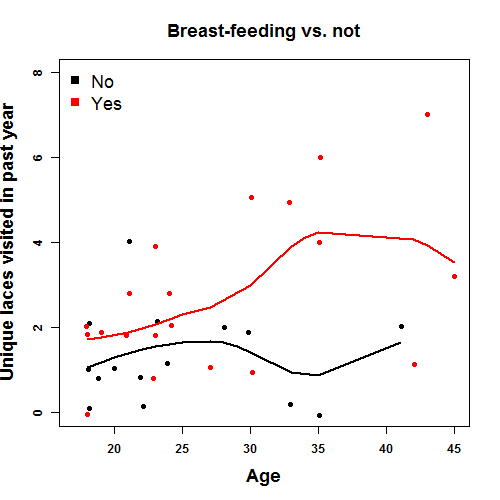
\includegraphics[width=0.75\textwidth]{bfeed_mob}
\caption{Please write your figure caption here}
\label{fig:1}       % Give a unique label
\end{figure}
>>>>>>> origin/master

\begin{table}
\caption{Missing data table}
\label{tab:miss_mr}  
\begin{tabular}{lllllllll}

\hline\noalign{\smallskip}
\multicolumn{9}{c}{Mental Rotations}\\
& & & Total & Missing & Practice & Performance & Other \\
\multicolumn{3}{l}{Women} & 64 & 21 & 10 & 7 & 4 \\
& \multicolumn{2}{l}{Post-Menopausal} & 16 & 11 & 6 & 2 & 3 \\
& \multicolumn{2}{l}{Reproductive-aged} & 43 & 10 & 4 & 5 & 1 \\
& & Breastfeeding & 27 & 6 & 2 & 3 & 1 \\
& & Not & 21 & 4 & 2 & 2 & 0 \\
\multicolumn{3}{l}{Men} & 65 & 11 & 5 & 4 & 2\\
\noalign{\smallskip}\hline

\hline\noalign{\smallskip}
\multicolumn{9}{c}{Corsi Blocks}\\
& & & Total & Missing & Practice & Performance & Other \\
\multicolumn{3}{l}{Women} & 54 & 16 & 2 & 9 & 5 \\
& \multicolumn{2}{l}{Post-Menopausal} & 13 & 7 & 2 & 2 & 3 \\
& \multicolumn{2}{l}{Reproductive-aged} & 41 & 8 & 0 & 7 & 1\\
& & Breastfeeding & 22 & 3 & 0 & 3 & 0 \\
& & Not & 19 & 5 & 0 & 4 & 1 \\
\multicolumn{3}{l}{Men} & 59 & 3 & 1 & 1 & 1\\
\noalign{\smallskip}\hline

\hline\noalign{\smallskip}
\multicolumn{9}{c}{Perspective Taking}\\
& & & Total & Missing & Practice & Performance & Other \\
\multicolumn{3}{l}{Women} & 64 & 35 & 33 & 0 & 2\\
& \multicolumn{2}{l}{Post-Menopausal} & 16 & 12 & 0 & 11 & 1 \\
& \multicolumn{2}{l}{Reproductive-aged} & 48 & 22 & 0 & 22 & 0\\
& & Breastfeeding & 27 & 12 & 0 & 12 & 0  \\
& & Not & 21 & 10 & 0 & 10 & 0 \\
\multicolumn{3}{l}{Men} & 65 & 13 & 12 & 0 & 1\\
\noalign{\smallskip}\hline

\hline\noalign{\smallskip}
\multicolumn{9}{c}{Pointing task}\\
& & & Total & Missing & Practice & Performance & Other \\
\multicolumn{3}{l}{Women} & 58 & 1 & 0 & 0 & 1 \\
& \multicolumn{2}{l}{Post-Menopausal} & 15 & 1 & 0 & 0 & 1 \\
& \multicolumn{2}{l}{Reproductive-aged} & 43 & 0 & 0 & 0 & 0 \\
& & Breastfeeding & 24 & 0 & 0 & 0 & 0 \\
& & Not & 19 & 0 & 0 & 0 & 0 \\
\multicolumn{3}{l}{Men} & 62 & & & & 1 \\
\noalign{\smallskip}\hline

\end{tabular}
\end{table}

The initial sample of 48 participants (40 reproductive aged and eight post-menopausal) was pared down at several stages before beginning analysis of mental rotation performance.  An additional two reproductive-aged women (ID: 13, 19) and three post-menopausal women (ID: 9, 38, 77) were unable to complete the task due to vision impairment.  An additional one post-menopausal women (ID: 78, 79) were unable to move beyond the practice stage and thus recorded no score on the task.  Finally, seven reproductive aged women (ID: 25, 26, 61, 75, 98, 99, 116) and two post-menopausal women (ID: 63, 103) who did complete the task had their scores dropped because they failed to exceed RANDOM?? performance and thus did not appear to understand the task.




	\subsection{Sex Differences}
	\label{sec:3.1}
The study enrolled 129 participants in total, with 65 men and 64 women.

		\subsubsection{Cognition and Navigation}		
		\label{sec:3.1.1}
In order to make scores easier to compare, all measure are re-coded such that a higher score indicates better performance on the task.		

\begin{table}
\caption{Sex differences (Cognition and navigation)}
\label{tab:sd_cog}  
\begin{tabular}{llll}
\hline\noalign{\smallskip}
DV & $M|F$ & Std. $\beta$ & Std. Err  \\
\noalign{\smallskip}\hline\noalign{\smallskip}
Acc & $55|43$ & .448* & .200 \\
RT & $55|43$ & -.149 & .204 \\
Span & $56|39$ & .224 & .208 \\
Persp & $52|29$ & .531* & .225 \\
Point & $62|57$ & .470* & .180 \\
\noalign{\smallskip}\hline
\end{tabular}
\end{table}

\paragraph{Mental Rotation}
The initial sample of 129 (65 men and 64 women) participants was pared down at several stages before beginning analysis of mental rotation performance.  Two men (ID: 22, 85) and four women (ID:9, 38, 77, 91) were unable to complete the task due to vision impairment.  An additional five men (ID: 21, 33, 107, 111) and ten women (ID: 34, 44, 61, 63, 71, 75, 78, 79, 99, 103) were unable to move beyond the practice stage and thus recorded no score on the task.  Finally, four men (ID: 16, 20, 76, 83) and seven women (ID: 1, 5, 11, 26, 42, 94, 118) who did complete the task had their scores dropped because they failed to exceed random performance and thus did not appear to understand the task.

As expected based on work in Western populations, previous work among the Twe, and the fertility and parental care hypothesis, men's responses in the mental rotation task were more accurate than women's.

\paragraph{Corsi Blocks}
The initial sample of 107 participants (59 men and 53 women) was pared down at several stages before beginning analysis of mental rotation performance.  One man (ID: 85) and five women (ID: 9, 13, 38, 77, 91) were unable to complete the task due to vision impairment.  An additional one man (ID: 111) and two women (ID: 78, 79) were unable to move beyond the practice stage and thus recorded no score on the task.  Finally, one man (ID: 24) and nine women (ID: 25, 26, 61, 63, 75, 98, 99, 103, 116) who did complete the task had their scores dropped because they failed to exceed RANDOM?? performance and thus did not appear to understand the task.  

There is no significant difference between Twe men's and women's performance on the Corsi Block task (see table).  However, this lack of finding is dependent on the decision to remove all participants who scored below two on the task.  If we instead work from the assumption that these participants did in fact understand the task but simply performed extremely poorly, there is a strong sex difference (report stats).

\paragraph{Perspective Taking}
One woman (ID: 38) and one man (ID: 85) were unable to complete the task due to vision impairment, and another woman abstained from the task because she was scared of the toy cheetah (ID: 42).  An additional 12 men (ID: 22, 24, 32, 40, 46, 65, 76, 84, 95, 107, 111, 114) and 33 women (ID: 3, 4, 8, 9, 11, 13, 25, 26, 31, 34, 37, 45, 49, 61, 63, 67, 71, 74, 75, 77, 78, 79, 86, 93, 94, 99, 103, 104, 105, 108, 109, 116, 126) were unable to move beyond the practice stage and thus recorded no score on the task.

Men performed significantly better on this task than women (see table), making smaller errors in setting the dial.

\paragraph{Pointing Accuracy}

One woman (ID: 38) and one man (ID: 85) were unable to complete the task due to vision impairment, and three men (ID: 2, 6, 112) and six women (ID: 1, 3, 4, 5, 7, 8) were unable to participate because the apparatus was unavailable at the time of their testing.

Three locations were dropped from the list because the majority of participants were not comfortable enough with their knowledge of the location to confidently indicate its bearing.  We arrived at a participant specific pointing accuracy score by averaging the error (i.e. difference between indicated and actual bearing to the location) across all attempted points.

Men pointed significantly more accurately to distant locations than women.

		\subsubsection{Anxiety}
		\label{sec:3.1.2}
Twenty-eight men and twenty-seven women responded to the harm avoidance questionnaire, and all but one of the men also responded to the spatial anxiety survey. 

Men recorded significantly lower scores on the spatial anxiety survey... Not on the harm avoidance...

\begin{table}
\caption{Sex differences (Anxiety)}
\label{tab:sd_anx}  
\begin{tabular}{llll}
\hline\noalign{\smallskip}
DV & $M|F$ & Std. $\beta$ & Std. Err  \\
\noalign{\smallskip}\hline\noalign{\smallskip}
SAX & $27|27$ & -0.745** & .255 \\
HA & $28|27$ & .-0.357 & .268 \\
\noalign{\smallskip}\hline
\end{tabular}
\end{table}

		\subsubsection{Mobility}
		\label{sec:3.1.2}
Forty-two men and forty-five women participated in the annual mobility interview. We are unable to calculate the percentage of trips made alone for two of those men and five of those women because these individuals did not spend the night anywhere outside their home village in the past year.  Twenty men and eighteen women carried trackers to measure daily movement.

\begin{table}
\caption{Sex differences (Mobility)}
\label{tab:sd_mob}  
\begin{tabular}{llll}
\hline\noalign{\smallskip}
DV & $M|F$ & Std. $\beta$ & Std. Err  \\
\noalign{\smallskip}\hline\noalign{\smallskip}
Visits & $42|45$ & .685** & .203 \\
Solo & $40|40$ & .565** & .216 \\
Daily & $20|18$ & .902** & .293 \\
\noalign{\smallskip}\hline
\end{tabular}
\end{table}

	\subsection{Fertile vs. non-fertile women}
	\label{sec:3.2}
Your text comes here. Separate text sections with

<<<<<<< HEAD
		\subsubsection{Cognition and Navigation}
		\label{sec:3.2.1}
The set of women above includes forty-three women of reproductive age and sixteen post-menopausal women.

\begin{table}
\caption{Menopausal effect (Cognition and navigation)}
\label{tab:fert_cog}  
\begin{tabular}{llll}
\hline\noalign{\smallskip}
DV & $Fert|Post-fert$ & Std. $\beta$ & Std. Err  \\
\noalign{\smallskip}\hline\noalign{\smallskip}
Acc & $38|5$ & -.386 & .478 \\
RT & $38|5$ & -1.194* & .444\\
Span & $33|6$ & -1.053* & .415 \\
Persp & $26|3$ & .059 & .621 \\
Point & $43|14$ & .189 & .309 \\
\noalign{\smallskip}\hline
\end{tabular}
\end{table}

\paragraph{Mental Rotation}
The initial sample of 59 participants was pared down at several stages before beginning analysis of mental rotation performance.  One reproductive-aged woman (ID: 91) and three post-menopausal women (ID: 9, 38, 77) were unable to complete the task due to vision impairment.  An additional four reproductive-aged women (ID: 44, 61, 75, 99) and six post-menopausal women (ID: 34, 63, 71, 78, 79, 103) were unable to move beyond the practice stage and thus recorded no score on the task.  Finally, five reproductive-aged women (ID: 1, 5, 26, 94, 118) and two post-menopausal women (ID: 11, 42) who did complete the task had their scores dropped because they failed to exceed random performance and thus did not appear to understand the task.

The post-menopausal ...  61.5\% of the women in the initial post-menopausal set were unable to pass out of either the practice set or perform above chance on the actual task, compared to 21.4\% of reproductive-aged women having similar issues.  This may be a sign of weakened spatial-cognitive ability, but it could also be due to some other factor.

\paragraph{Corsi Blocks}
The initial sample of 48 participants (40 reproductive aged and eight post-menopausal) was pared down at several stages before beginning analysis of mental rotation performance.  An additional two reproductive-aged women (ID: 13, 19) and three post-menopausal women (ID: 9, 38, 77) were unable to complete the task due to vision impairment.  An additional two post-menopausal women (ID: 78, 79) were unable to move beyond the practice stage and thus recorded no score on the task.  Finally, seven reproductive aged women (ID: 25, 26, 61, 75, 98, 99, 116) and two post-menopausal women (ID: 63, 103) who did complete the task had their scores dropped because they failed to exceed RANDOM?? performance and thus did not appear to understand the task.

\paragraph{Perspective Taking}
One post-menopausal woman (ID: 38) was unable to complete the task due to vision impairment, and another woman abstained from the task because she was scared of the toy cheetah (ID: 42).  An additional 12 men (ID: 22, 24, 32, 40, 46, 65, 76, 84, 95, 107, 111, 114) and 33 women (ID: 3, 4, 8, 9, 11, 13, 25, 26, 31, 34, 37, 45, 49, 61, 63, 67, 71, 74, 75, 77, 78, 79, 86, 93, 94, 99, 103, 104, 105, 108, 109, 116, 126) were unable to move beyond the practice stage and thus recorded no score on the task.

\paragraph{Pointing Accuracy}

One woman (ID: 38) and one man (ID: 85) were unable to complete the task due to vision impairment, and three men (ID: 2, 6, 112) and six women (ID: 1, 3, 4, 5, 7, 8) were unable to participate because the apparatus was unavailable at the time of their testing.

		\subsubsection{Anxiety}
		\label{sec:3.2.2}
Your text comes here. Separate text sections with	

\begin{table}
\caption{Menopausal effect (Anxiety)}
\label{tab:fert_anx}  
\begin{tabular}{llll}
\hline\noalign{\smallskip}
DV & $Fert|Post-fert$ & Std. $\beta$ & Std. Err  \\
\noalign{\smallskip}\hline\noalign{\smallskip}
SAX & $19|8$ & -.740. & .404 \\
HA & $19|8$ & .019 & .430 \\
\noalign{\smallskip}\hline
\end{tabular}
\end{table}

		\subsubsection{Mobility}
		\label{sec:3.2.3}
Your text comes here. Separate text sections with	

\begin{table}
\caption{Menopausal effect (Mobility)}
\label{tab:fert_mob}  
\begin{tabular}{llll}
\hline\noalign{\smallskip}
DV & $Fert|Post-fert$ & Std. $\beta$ & Std. Err  \\
\noalign{\smallskip}\hline\noalign{\smallskip}
Visits & $35|10$ & -.342 & .359 \\
Solo & $30|10$ & .389 & .365 \\
Daily & $15|3$ & 1.240* & .574 \\
\noalign{\smallskip}\hline
\end{tabular}
\end{table}

	\subsection{Fertile women with/without young dependents}
	\label{sec:3.3}
Your text comes here. Separate text sections with

		\subsubsection{Cognition and Navigation}
		\label{sec:3.3.1}
Your text comes here. Separate text sections with	

\begin{table}
\caption{Post-partum effect (Cognition and navigation)}
\label{tab:bf_cog}  
\begin{tabular}{llll}
\hline\noalign{\smallskip}
DV & $BF|NBF$ & Std. $\beta$ & Std. Err  \\
\noalign{\smallskip}\hline\noalign{\smallskip}
Acc & $24|14$ & .033 & .341 \\
Acc.5 & $21|13$ & .162 & .357 \\
RT & $24|14$ & .037 & .341 \\
RT.5 & $21|13$ & -.105 & .358 \\
Span & $21|14$ & .079 & .350 \\
Span2 & $18|11$ & -.030 & .390 \\
Persp & $15|8$ & .168 & .447 \\
Point & $24|14$ & .526 & .330 \\
\noalign{\smallskip}\hline
\end{tabular}
\end{table}

		\subsubsection{Anxiety}
		\label{sec:3.3.2}
Your text comes here. Separate text sections with	

\begin{table}
\caption{Post-partum effect (Anxiety)}
\label{tab:bf_anx}  
\begin{tabular}{llll}
\hline\noalign{\smallskip}
DV & $BF|NBF$ & Std. $\beta$ & Std. Err  \\
\noalign{\smallskip}\hline\noalign{\smallskip}
SAX & $12|7$ & 1.082* & .413 \\
HA & $12|7$ & .281 & .485 \\
\noalign{\smallskip}\hline
\end{tabular}
\end{table}

		\subsubsection{Mobility}
		\label{sec:3.3.3}
Your text comes here. Separate text sections with	

\begin{table}
\caption{Post-partum effect (Mobility)}
\label{tab:bf_mob}  
\begin{tabular}{llll}
\hline\noalign{\smallskip}
DV & $BF|NBF$ & Std. $\beta$ & Std. Err  \\
\noalign{\smallskip}\hline\noalign{\smallskip}
Visits & $20|11$ & 1.049** & .328 \\
Solo & $19|7$ & .015 & .451 \\
Daily & $7|7$ & -.162 & .554 \\
\noalign{\smallskip}\hline
\end{tabular}
\end{table}
		
% For one-column wide figures use
\begin{figure}[!htb]
  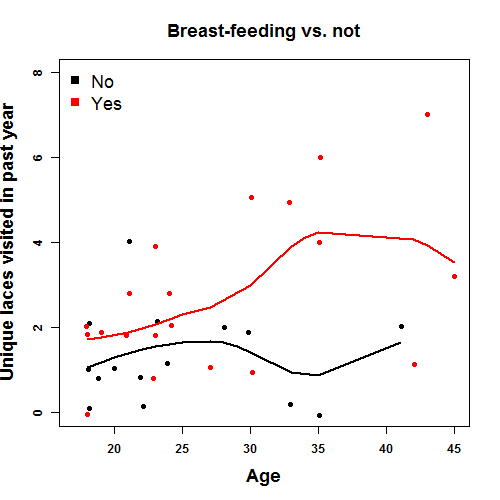
\includegraphics[width=0.75\textwidth]{bfeed_mob}
\caption{Please write your figure caption here}
\label{fig:1}       % Give a unique label
\end{figure}


=======
>>>>>>> origin/master
\section{Discussion}
\label{sec:4}
Text with citations \cite{RefB} and \cite{RefJ}.

%
% For two-column wide figures use
\begin{figure*}
  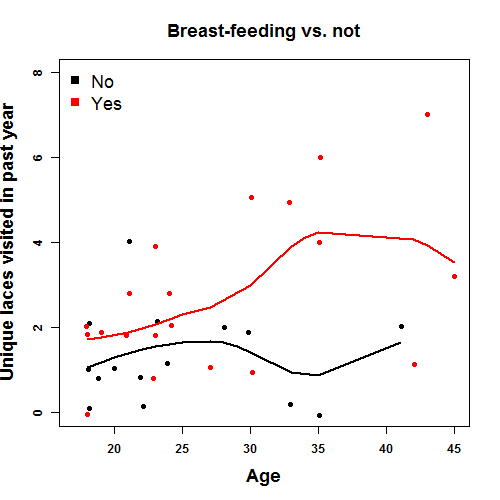
\includegraphics[width=0.75\textwidth]{bfeed_mob}
\caption{Please write your figure caption here}
\label{fig:2}       % Give a unique label
\end{figure*}
%



%\begin{acknowledgements}
%If you'd like to thank anyone, place your comments here
%and remove the percent signs.
%\end{acknowledgements}

% BibTeX users please use one of
%\bibliographystyle{spbasic}      % basic style, author-year citations
%\bibliographystyle{spmpsci}      % mathematics and physical sciences
%\bibliographystyle{spphys}       % APS-like style for physics
%\bibliography{}   % name your BibTeX data base

% Non-BibTeX users please use
\begin{thebibliography}{}
%
% and use \bibitem to create references. Consult the Instructions
% for authors for reference list style.
%
\bibitem{RefJ}
% Format for Journal Reference
Author, Article title, Journal, Volume, page numbers (year)
% Format for books
\bibitem{RefB}
Author, Book title, page numbers. Publisher, place (year)
% etc
\end{thebibliography}

\end{document}
% end of file template.tex

